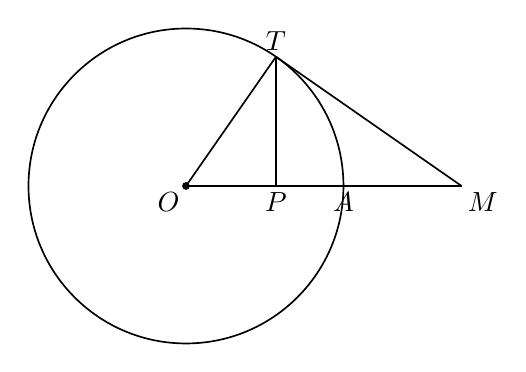
\begin{tikzpicture}[x=1cm,y=1cm,line width=.6pt,font=\normalsize]
\coordinate (O) at (0,0);
\coordinate (P) at (1.14285714,0);
\coordinate (A) at (2,0);
\coordinate (M) at (3.5,0);
\coordinate (T) at (1.14285714,1.64130361);
\draw (O) circle[radius=2cm];
\draw (O)--(M);
\draw (O)--(T);
\draw (T)--(M);
\draw (T)--(P);
\node[below left=2pt,inner sep=0pt] at (O) {$O$};
\node[below=2pt,inner sep=0pt] at (P) {$P$};
\node[below=2pt,inner sep=0pt] at (A) {$A$};
\node[below right=2pt,inner sep=0pt] at (M) {$M$};
\node[above=2pt,inner sep=0pt] at (T) {$T$};

% Explicit named circle-center points, painted after all region fills.
\fill (O) circle[radius=1.4pt];
\end{tikzpicture}
